\documentclass[a4paper,10pt]{article}
\usepackage[english]{babel}
\usepackage[utf8]{inputenc}
\usepackage[toc,page]{appendix}
\usepackage{graphicx}

%Includes "References" in the table of contents
\usepackage[nottoc]{tocbibind}
\usepackage{titling}
\usepackage{setspace}

\usepackage{graphicx}
\parskip .8ex

%\setlength{\droptitle}{-15em} %%%% Add this line if need more space. %%%%

%Begining of the document
\begin{document}

\title{CSCM38: Adv Topic - Artificial Intelligence and Cyber Security - Coursework 1}
\author{Andy Gray\\445348}
\date{10/11/2020}

\maketitle

\section{Introduction}
\label{sec:intro}
	We will be looking at some issues surrounding an advanced topic within natural language processing (NLP).  NLP is a form of artificial intelligence  (AI) that aims to as the automatic manipulation of natural language, like speech and text, by software \cite{nlp_definition}. However, human language is highly ambiguous, ever-changing and evolving. People are great at producing language and understanding language, allowing them to be capable of communicating, perceiving, and understanding very complex and nuanced meanings. At the same time, while we humans are great users of language, we are also not very good at formally recognising and explaining the rules that dictate our language \cite{goldberg2017neural}. So if the human language is difficult for humans, the process, therefore, can not be straight forward for computers either. However, some advancements over the years, like sentiment analysis has allowed us to analyse general moods, and speech-to-text has genuinely revolutionised the way people can interact and create documents.  
	
	A Swiss linguistics professor in the 1900s, Ferdinand de Saussure, created the concept of "Language as a Science \cite{koerner2013ferdinand}." However, Professor Saussure, around 1911, offered three courses at the University of Geneva. At this university is where it got developed as a proposal for describing languages as "systems." Within the language, a sound represents a concept, a concept that shifts its meaning as the context changes \cite{nlp_history}. It was not until the 1950s where a British mathematician named Alan Turing wrote a paper, laying out a test for a "thinking" machine. In his paper, he said that if a machine could be part of a conversation, and it imitated a human so well that there were no noticeable differences. The machine could be considered capable of thinking \cite{turing2004can}. However, the Hodgkin-Huxley model showed how the brain uses neurons in forming an electrical network. These events helped inspire the idea of AI, NLP, and the evolution of computers \cite{nlp_history}.
	
	In 1957 previous linguistic concepts got revolutionised, concluding that for a computer to understand a language, the sentence structure would have to be changed \cite{chomsky2002syntactic}. These revolutions created the style of grammar called Phase-Structure Grammar, which methodically translated natural language sentences into a format that is usable by computers \cite{nlp_history}. 
	
	In the 1960s is when research into AI and NLP stopped due to the technology not being where it needed to be and costing more than hiring people to translate \cite{nlp_history}. It took until the 1980s for NLP and AI \cite{what_ai} research to resume after the failed expectations in the earlier years \cite{nlp_history}. However, it was not until the 1990s, where statistical models for NLP popularity started to grow. The pure statistics NLP methods have become remarkably valuable in keeping pace with the vast amounts of online text \cite{nlp_history}. N-Grams have become useful, recognising and tracking clumps of linguistic data, numerically \cite{n_grams}. In 1997, LSTM and recurrent neural net (RNN) models \cite{nlp_rnn} were introduced and found their niche in 2007 for voice and text processing. Currently, neural net models are considered the cutting edge of research and development in the NLP's understanding of text and speech generation \cite{nlp_history}.
	
	%[Explain/ overview of how NN have become good at NLP]\\
	With the growth of RNN, these helped advance the field of NLP with ML. However, it got quickly found out that they had several issues, including the vanishing gradient problem, and that it only has a short term memory. This problem brought about the introduction of LSTMs, and then later a simplified version called a Gated Recurrent Units (GRU). With the introduction of RNN and the growth with popularity with frameworks like TensorFlow and PyTorch. We will be proposing a project plan that will be looking at LSTMs and GRU cells to see which one performs better on a given dataset about natural disasters \cite{disater_kaggle} using the TensorFlow deep learning library \cite{tensorflow}. As when we are creating a model for real-world deployment, not only does the model need to have a high level of accuracy and do what gets expected of it, in regards to the end-users expectations, but it also has to do it quickly.
	
	%[overview of what to expect in assignment]\\
	First, we will look into the related work, covering what NLP is and some of its overviews, then we will look at the more recent advancements of NLP and look into how they work and some of their drawbacks. These techniques include RNN, LSTMs and GRU. Additionally, we will be looking at what advantages they are claiming to have over each other. Then finally, we will be overviewing the aims of the proposed project and how it intends to compare the different RNN model's cells for training speed, accuracy and the validation loss values, the RMSE and MAE values.
	

\section{Related Work}
\label{sec:related_work}

	ML for NLP and text analytics involves using ml algorithms and "narrow" AI \cite{ml_nlp}. These approaches allow the computer to understand the meaning of text documents, which can be about anything that contains the text. Some examples include social media comments, online reviews, survey responses, even financial, medical, legal and regulatory documents. Therefore the aim of ML and AI in NLP is to improve, accelerate and automate the underlying text analytics functions and NLP features that turn any given unstructured text into useable data and insights \cite{ml_nlp}.
	
	Generally speaking, NLP breaks down the language into shorter, more basic pieces. These shorter pieces are called tokens which can get made up of words and periods, for example. The NLP will then attempt to understand the relationships of the tokens, which the process often uses higher-level NLP features, such as \cite{nlp_history} content Categorisation, which is a process that creates a linguistic document summary that includes content alerts, duplication detection, search, and indexing. Topic Discovery and Modeling that aims to capture the themes and meanings of text collections and applies advanced analytics to the text. Another process is that contextual extraction, which will automatically pull structured data from text-based sources. Sentiment Analysis aims to identify the general mood, or subjective opinions, stored in large amounts of text. Useful for opinion mining. Text-to-Speech and Speech-to-Text Conversion process aim to transform voice commands into text, and vice versa. Document summarisation is a process that automatically creates a synopsis, condensing large amounts of text. Machine Translation is another process that automatically translates the text or speech of one language into another.

%\subsection{Traditional ML Approaches}

%The most popular supervised NLP machine learning algorithms are \cite{ml_nlp}:
%Support Vector Machines
%Bayesian Networks
%Maximum Entropy
%Conditional Random Field

\subsection{Recurrent NN (RNN) for NLP}

	A recurrent neural network (RNN), at its most fundamental level, is simply a type of densely connected neural network (NN). However, the main difference to a dense fully connected NN and an RNN is the introduction of time into the model. What this means is that the output of the hidden layer in an RNN gets fed back into itself \cite{adv_in_ml, geron2019hands}.
	
	\begin{figure}
		\begin{center}
			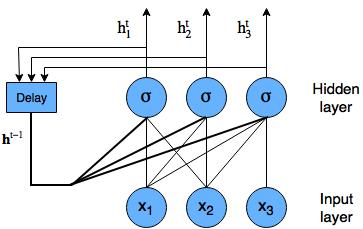
\includegraphics[width=7cm]{explicit_RNN.jpg}
			\caption{A reprentation of a RNN \cite{adv_in_ml}}
			\label{fig:rnn_diagram}
		\end{center}
	\end{figure} 
	
	In fig: \ref{fig:rnn_diagram}, we have a simple RNN, also referred to as a vanilla RNN \cite{geron2019hands}, which has three input nodes. As usually expected in a dense NN, the hidden layers have sigmoid activation functions, from the output of each previous layer. However, where an RNN changes to a dense NN is that the output of the hidden layer then gets fed back into the same hidden layer. This step allows the hidden layer outputs to get passed through a conceptual delay block to allow the input of $h^{t-1}$ into the hidden layer. By doing this within the RNN, it allows the model to be able to model time or sequence-dependent data \cite{adv_in_ml, geron2019hands}.
	
	RNN are very flexible \cite{geron2019hands}. In the implementation shown in fig: \ref{fig:m2m_rnn_diagram}, we have a many-to-many model. What this means is that we have the input sequence "A girl walked into a bar…" and we also have many outputs. These outputs can be notated as $h_0$ to $h_t$ \cite{adv_in_ml}. However, we can also have other setups, for example, one-to-many and many-to-one \cite{jjslides}.  One-to-many is the process of supplying one input and predicting multiple outputs. What this approach is trying to do is to generate sentences based on a single input, or a single word. Additionally, a many-to-one is the process of supplying many words as input, like the sentence, and the model will then predict the next word \cite{adv_in_ml}.
	
	\begin{figure}
		\begin{center}
			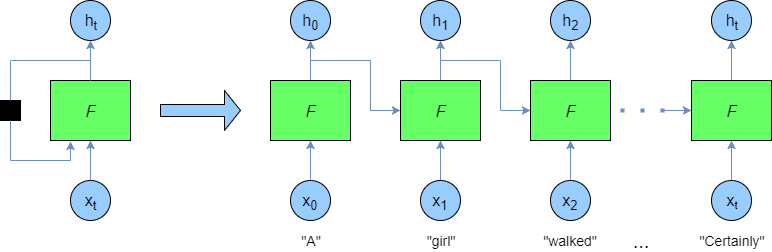
\includegraphics[width=9cm]{Recurrent-neural-network.png}
			\caption{A reprentation of a many to many RNN \cite{adv_in_ml}}
			\label{fig:m2m_rnn_diagram}
		\end{center}
	\end{figure} 
	
	However, one thing to take into account is that a vanilla RNN does not get used often in practice \cite{grus2019data}. One of the reasons being is the vanishing gradient problem \cite{geron2019hands}. The vanishing gradient is where the contribution from the earlier steps becomes insignificant in the gradient descent step \cite{rnn_lstm_explained}. For RNN to work effectively, we would want to have long memories. We would want this longer-term memory so the network can connect data relationships at significant distances in time, therefore having a more extended memory than currently on offer. Due to the lack of long term memory RNN get referred to as a short term memory network. Long term memory networks could make real progress in understanding how language and narrative works or how stock market events get correlated, for example. However, due to the limitations of the RNN, the more time steps we have, the more possibility we have of back-propagation gradients either accumulating and exploding or vanishing down to nothing \cite{adv_in_ml}. The exploding gradient happens when the algorithm assigns high importance to the weights, without much reason. However, this problem can be solved by truncate or squash the gradients \cite{rnn_lstm_explained}.
	
%\subsection{BERT for NLP}

\subsection{LSTM for NLP}
	
	Long Short-Term Memory (LSTM) is a specific RNN architecture that got designed to model temporal sequences and their long-range dependencies more accurately than conventional RNNs \cite{sak2014long, grus2019data}. LSTM RNNs have shown to be more effective than Deep NNs (DNNs) and conventional RNNs. Especially for acoustic modelling \cite{sak2014long}. LSTM cell got first proposed in 1997 \cite{hochreiter1997long} but has gradually got improved over the years \cite{geron2019hands, sak2014long, zaremba2014recurrent}.  
	
	How LSTM works is that the cell within the RNN has two vectors, $h_{(t)}$ and $c_{(t)}$. Therefore the best way to think of this is that $c$ the cell, $c_{(t)}$ is the long term state and $h_{(t)}$ is the short term state \cite{geron2019hands}. When visually conceptualising the network, all RNN have the form of a chain of repeating modules of NN. In vanilla RNNs, this repeating module will have a straightforward structure, such as a single tanh layer. LSTMs also have this chain-like structure. However, instead of having a single NN layer, LSTM has four, interacting in a very different way to a vanilla RNN \cite{lstm_networks}. 
	
	\begin{figure}
		\begin{center}
			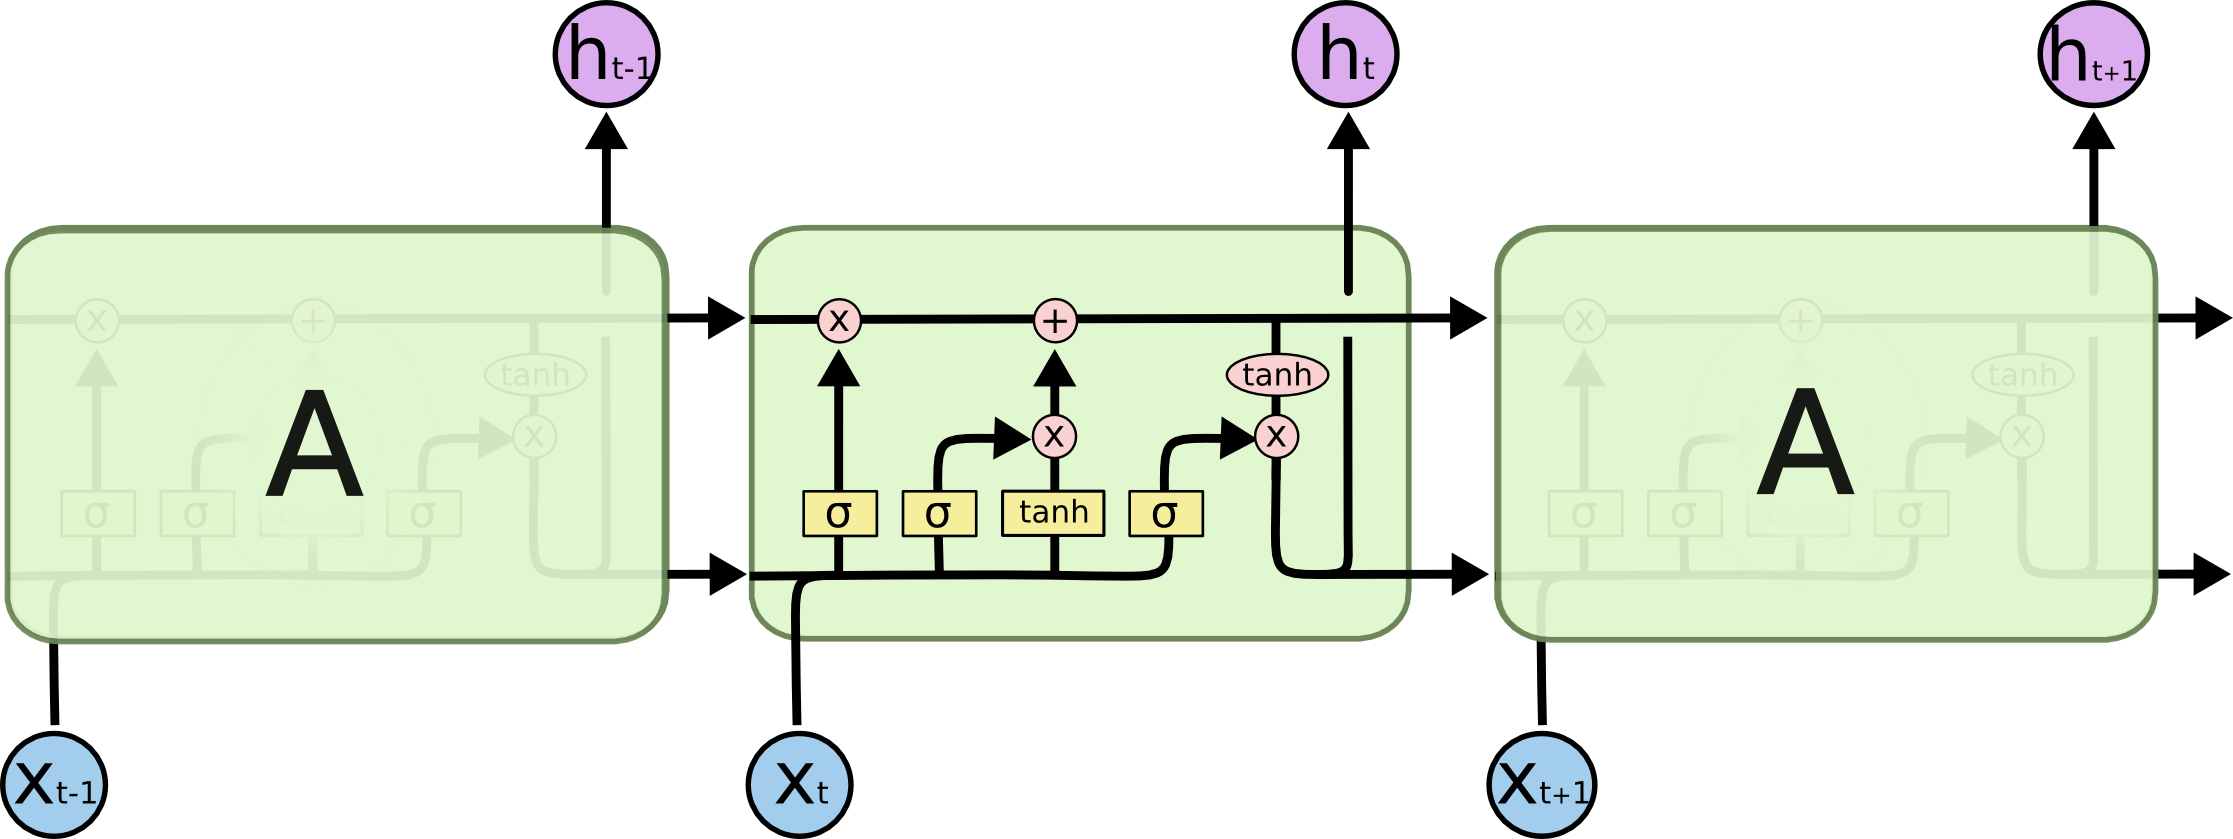
\includegraphics[width=9cm]{LSTM3-chain.png}
			\caption{A reprentation of a many to many RNN \cite{lstm_networks}}
			\label{fig:LSTM_diagram}
		\end{center}
	\end{figure} 
	
	The key to LSTMs is the cell state, the horizontal line running through the top of the diagram (see fig: \ref{fig:LSTM_diagram}). The cell state runs straight down the entire chain, with only some minor linear interactions. They are therefore allowing for the information to flow through the cells, unchanged if needed. However, LSTM does have the ability to remove or add information to the cell state. 
	
	These changes get done by the structures called gates. Gates are a way to let information through optionally, depending on the criteria set, which get formed out of a sigmoid NN layer and a pointwise multiplication operation \cite{lstm_networks}. The sigmoid layer outputs numbers between zero and one, describing how much of each element should get let through. A value of zero means will let nothing through, while a value of one means everything will get through \cite{lstm_networks, geron2019hands}. An LSTM has three of these gates, to protect and control the cell state \cite{lstm_networks}. The three gates are a forget gate, input gate, and output gate \cite{illustrated_lstm_gru, geron2019hands}. The forget gate, which is controlled by the $f_{(t)}$ determines what part of the long-term state should get forgotten. While the input gate, controller by the $i_{(t)}$, decides on which parts of $g_{(t)}$ should get added to the long-term state. Then the output gate, controlled by the $o_{(t)}$ figures out what part of the long-term state should be read and outputted through the time step, both to $h_{(t)}$ and $y_{(t)}$ \cite{geron2019hands}.
	
	Overall an LSTM RNN will perform better than a vanilla RNN.  Training will converge faster, and it will detect long-term dependencies in the data \cite{geron2019hands}. LSTMs have made remarkable developments in the fields of language modelling, text generation, Image processing, speech and handwriting recognition, music generation and language translation \cite{g4g}. However, LSTMs do have a few drawbacks \cite{g4g}. While LSTMs became popular because they can solve the vanishing gradient, which they can, they do not though remove it altogether. The problem gets caused by the model still having to move data from one cell to another. Another drawback is that they require a lot of resources and time to train. Additionally, with the rise of big data, developers are looking for a model that can remember the context for a lot longer than what LSTMs can now. LSTMs can be prone to overfitting and can get affected easily by different random weight initialisations.
	
\subsection{GRU for NLP}

	\begin{figure}
		\begin{center}
			\includegraphics[width=9cm]{GRU_example.png}
			\caption{A reprentation of GRU cell \cite{illustrated_lstm_gru}}
			\label{fig:gru_example}
		\end{center}
	\end{figure}

	GRU stands for Gated Recurrent Units, and despite being quite similar to LSTMs, they are, however, a more simplified version of the cell \cite{geron2019hands, grus2019data}. GRUs have never been as popular as they are now \cite{g4g, geron2019hands}. However, GRUs are a simpler cell compared to an LSTM but perform just as well as the LSTM \cite{greff2016lstm}. GRUs are an RNN that have a gated mechanism to obtain dependencies of different time scales as effectively and adaptively as possible \cite{cho2014learning}. 
	
	GRUs have an update gate, and a reset gate (see fig: \ref{fig:gru_example}), which is responsible for selecting what information is to get taken forward and the rest gate is in between the two successive recurrent units. This gate decides on how much information needs to get forgotten. A single gate controller $z_{(t)}$ controls the forget and the input gate \cite{geron2019hands}.  Another striking aspect of GRUs is that they do not store cell state in any way. Therefore, there is no output gate. The full state vector gets outputted at every time step \cite{geron2019hands}. Therefore they are unable to control how much memory the next unit will get given \cite{g4g}.    
	
	GRUs provide most of the same benefits of LSTMs but have fewer tensor operations and are therefore a little speedier to train then LSTMs \cite{illustrated_lstm_gru}. While GRUs are a crucial reason RNN are a success at NLP, they do however have limited short-term memory and also have difficulty learning long-term patterns in sequences of 100-time steps or above \cite{geron2019hands}.


\section{Project Plan}
\label{sec:project_plan}

	While both GRUs have their benefits and drawbacks, there is not a clear winner which one is better. Researchers and engineers usually try both to determine which one works better for their use case \cite{illustrated_lstm_gru}. So with this in mind, we are proposing an experiment to determine which one is better at a classification of text problem. We aim to see which one performs better for the provided NLP dataset out of an LSTM and GRU.
	
	We want to be able to see what are the noticeable differences or benefits over using an LSTM over a GRU or vice versa. We will be using the "Real or Not? NLP with Disaster Tweets \cite{disater_kaggle}" dataset to test the two RNN cell types.  The data has two CSV files, training and testing. However, we will be using the training dataset only and splitting this data.
	The training dataset contains the text of a tweet; a keyword from that tweet; the location the tweet got sent. However, we must note that some of this information might be blank, and some of these attributes might get discarded during the preprocessing stage. While the network aim is to predict if the given tweet is tweeting about a real disaster, with a "1" label, or not, "0" label. 
	
	In order to decide on what cell performed better, we will be using several metrics. The metrics that will get used to comparing the different cells are the time it takes to train the network, the training loss and validation loss values, the RMSE and MAE values. We also intended to train and run the experiment at least five times with each changed parameters of the networks, and this is to allow us to see if there is a consistent trend within the results or if they change depending on the set parameters used.
	
	
\medskip
\newpage
%\begin{appendices}
	
	
%\end{appendices}

%\newpage

%Sets the bibliography style to UNSRT and imports the 
%bibliography file "samples.bib".
\bibliographystyle{acm}
\bibliography{samples}

\end{document}